%%%%%%%%%%%%%%%%%%%%%%%%%%%%%%%%%%%%%%%%%
%  Telemac Documentation
%  Example of the TelemacDoc class
%
%%%%%%%%%%%%%%%%%%%%%%%%%%%%%%%%%%%%%%%%%

%----------------------------------------------------------------------------------------
%	PACKAGES AND OTHER DOCUMENT CONFIGURATIONS
%----------------------------------------------------------------------------------------
\documentclass[Courlis]{../../data/TelemacDoc} % Default font size and left-justified equations
%\documentclass[Courlis,french]{TelemacDoc} % Default font size and left-justified equations in french

%%---------------------------------------------------------------------------
%% Command for COURLIS names
%%---------------------------------------------------------------------------
\newcommand{\Cbedload}{{\scshape Courlis-bedload}\xspace}
\newcommand{\Csuspension}{{\scshape Courlis-suspension}\xspace}
\newcommand{\fudaa}{{\scshape Fudaa-Mascaret}\xspace}
\newcommand{\precourlis}{{\scshape PreCourlis}\xspace}
\newcommand{\cas}{\telfile{cas file}\xspace}
\newcommand{\cass}{\telfile{cas files}\xspace}
\newcommand{\xcas}{\telfile{xcas file}\xspace}
\newcommand{\xcass}{\telfile{xcas files}\xspace}
%%---------------------------------------------------------------------------
%% Nomenclature
%%---------------------------------------------------------------------------
\usepackage{ifthen}
\usepackage{nomencl}
%
\makenomenclature
\renewcommand{\nompreamble}{\markboth{%
                            \MakeUppercase\nomname}{\MakeUppercase\nomname}%
                           }
\newcommand{\nomunit}[1]{%
\renewcommand{\nomentryend}{\hspace*{\fill}#1}}
% \usepackage{subcaption} % Not compatible with subfig
\definecolor{codegreen}{rgb}{0,0.6,0}
\definecolor{codegray}{rgb}{0.5,0.5,0.5}
\definecolor{codepurple}{rgb}{0.58,0,0.82}
\definecolor{backcolour}{rgb}{0.95,0.95,0.92}

\lstdefinestyle{mystyle}{
    backgroundcolor=\color{backcolour},
    commentstyle=\color{codegreen},
    keywordstyle=\color{magenta},
    numberstyle=\tiny\color{codegray},
    stringstyle=\color{codepurple},
    basicstyle=\ttfamily\scriptsize,
    breakatwhitespace=false,
    breaklines=true,
    captionpos=b,
    keepspaces=true,
    numbers=left,
    numbersep=5pt,
    showspaces=false,
    showstringspaces=false,
    showtabs=false,
    tabsize=2
}

\lstset{style=mystyle}

\lstdefinelanguage{TelemacCasRed}{
  basicstyle=\ttfamily\footnotesize,
  commentstyle=\color{PantoneRed},
  morecomment=[f]{/},
}
%----------------------------------------------------------------------------------------

\begin{document}

\let\cleardoublepage\clearpage

%----------------------------------------------------------------------------------------
%	TITLE PAGE
%----------------------------------------------------------------------------------------
\title{\courlis}
\subtitle{User Manual}
\version{\telmaversion}
\date{\today}
\maketitle
\clearpage


%----------------------------------------------------------------------------------------
%	COPYRIGHT PAGE
%----------------------------------------------------------------------------------------

\newpage

\thispagestyle{empty}

\TelemacCopyright{}


%----------------------------------------------------------------------------------------
%	TABLE OF CONTENTS
%----------------------------------------------------------------------------------------


\pagestyle{empty} % No headers

\tableofcontents% Print the table of contents itself

%\cleardoublepage % Forces the first chapter to start on an odd page so it's on the right

\pagestyle{fancy} % Print headers again

\printnomenclature

%----------------------------------------------------------------------------------------
%	Introduction
%----------------------------------------------------------------------------------------
\addcontentsline{toc}{section}{Introduction}
\chapter*{Introduction}\label{intro}

The one-dimensionnal hydro-sedimentary code \courlis is designed to simulate sediment transport in rivers and reservoirs where the flows can be considered as 1D. It is weakly coupled with the one-dimensionnal hydrodynamic software \mascaret. Both are part of the open-source system \telemacsystem (\texttt{www.opentelemac.org}).

\begin{figure}[htb!]
    \centering
    \includegraphics[width=\textwidth]{./graphics/telemac.png}
    \caption{\courlis within the \telemacsystem}
    \label{fig:telemac}
\end{figure}

The software supports steady and unsteady flow computations thanks to the three computational kernels of \mascaret :
\begin{itemize}
	\item SARAP : the steady flow kernel for subcritical, supercritical or mixed flow regimes (finite differences)
	\item REZO : the unsteady subcritical flow kernel (finite differences)
	\item MASCARET : the unsteady trans-critical flow kernel (finite volumes)
\end{itemize}
Complete description of those kernels can be found in the \mascaret guides. \mascaret computes surface elevations, discharge and velocities along the bief. These variables are then passed to the module \courlis to calculate sediment transport capacity and bed evolutions.  

Two options are available in \courlis to model sediment transport : 
\begin{itemize}
	\item Modelling suspended load : the sediment particles are transported by the flow and maintained (possibly temporary) in suspension above the bottom by the action of shear stress at bottom. 
	\item Modelling bedload : the sediment particles are transported in direct contact with the bottom or next to the bed without being affected by the fluid turbulence.
\end{itemize}
In physical systems, both mechanisms are generally observed but their mathematical representation are quite different. In \courlis suspended load is the solution of an advection-diffusion equation with erosion and deposition fluxes while bedload is estimated thanks to closure relantionships for sediment transport capacity and a continuity equation for the bed (Exner equation). 

\begin{figure}[htb!]
    \centering
    \includegraphics[width=.8\textwidth]{./graphics/transport_mechanisms.png}
    \caption{Sketch summarizing sediment transport mechanisms - saltation can be modeled with both bedload and suspended load modules (extracted from \cite{univ_lyon})}
    \label{fig:mechanisms}
\end{figure}

\Csuspension model both cohesive (fine particles such as silt or clay) or non-cohesive sediment (sand). 
\Cbedload is usually used to model gravel or coarse sand transport. 

\begin{figure}[htb!]
    \centering
    \includegraphics[width=0.8\textwidth]{./graphics/sediment_sizes.png}
    \caption{Canadian system soil classification also called SCCS classification (1987)}
    \label{fig:sediment_sizes}
\end{figure}






\newpage
%----------------------------------------------------------------------------------------
%	CHAPTER 1: Theoretical aspects
%----------------------------------------------------------------------------------------
\chapter{Theoretical aspects}\label{chap1}
\section{Hydrodynamics}
\mascaret solves the shallow water equations for incompressible flow, hydrostatic pressure and uniform distribution of velocities along the vertical axis. The flow slope and the horizontal curvature radius are supposed low. Wind effects on the free surface are also neglected. Flow is described on each section through mean velocity and mean free surface elevation.

\begin{CommentBlock}{Limit} 
	To use \courlis, only one reach can be considered. Besides, only the main channel can be taken into account and no singularities can be modeled.
\end{CommentBlock}

%%%%%%%%% ST VENANT %%%%%%%%%
\subsection{Shallow water equations}
The shallow water equations with variable section are given below :
\bequ
    \left\{
        \begin{array}{ll}
            \frac{\partial S}{\partial t} + \frac{\partial Q}{\partial x} = q_l\\
            \frac{\partial Q}{\partial t} + \frac{\partial \beta \frac{Q^2}{S}}{\partial x} + gZ\left( \frac{\partial Z}{\partial x} +J\right)= \frac{Q}{S} q_l\\
        \end{array}
    \right.
    \label{eq:shallow}
\eequ

with :
\begin{itemize}
	\item $S$ the wetted area ;
	\item $q_l$ the lateral inflows (confluence) in $m^2.s^{-1}$ ;
	\item $Q$ the mean discharge across the section ;
	\item $Z$ the free surface elevation ;
	\item $g$ the acceleration due to gravity ;
	\item $J$ the mean energy dissipation rate ;
	\item $\beta$ accounts for the variations of the real flow velocity accross the section \cite{mascaret_guide}.
\end{itemize}

\nomenclature{$S$}{Wetted area \nomunit{$m^2$}}
\nomenclature{$t$}{Time \nomunit{$s$}}
\nomenclature{$x$}{Longitudinal space variable \nomunit{$m$}}
\nomenclature{$q_l$}{Lateral inflows \nomunit{$m^2.s^{-1}$}}
\nomenclature{$g$}{Gravity acceleration \nomunit{$m^2.s^{-1}$}}
\nomenclature{$Q$}{Mean discharge accross the section \nomunit{$m^3.s^{-1}$}}
\nomenclature{$Z$}{Mean free surface elevation across the section \nomunit{$m$}}
\nomenclature{$J$}{Mean energy dissipation rate or energy slope \nomunit{$m.m^{-1}$}}

%%%%%%%%% RUGOSITE %%%%%%%%%
\subsection{Friction}
Bed and shores shear stress is taken into account through the Strickler friction law :
\bequ
	J = \frac{Q^2}{S^2 K^2 R_h^{\frac{4}{3}}}
	\label{eq:strickler}
\eequ
where :
\begin{itemize}
	\item $K$ is the Strickler coefficient ;
	\item $R_h$ the hydraulic radius.
\end{itemize}

The local shear stress $\tau_{tot}$ is computed by :

\bequ
	\tau_{tot} = \rho_w g R_h J = \frac{\rho_w g U^2}{K^2 R_h^{\frac{1}{3}}}
	\label{eq:contrainte_totale}
\eequ
For real cases, the hydraulic radius is usually approximated by the mean water depth across the section : $R_h \sim H$.
This option is activated by default in \courlis. 

\nomenclature{$H$}{Mean water depth across the section \nomunit{$m$}}
\nomenclature{$K$}{Strickler coefficient \nomunit{$m^{\frac{1}{3}}.s^{-1}$}}
\nomenclature{$R_h$}{Hydraulic radius \nomunit{$m$}}

%%%%%%%%% PLANIMETRAGE %%%%%%%%%
\subsection{Vertical discretization}
\label{planim}

Vertical discretization is used to transform cross-sections (2D) to unidimensional variables. Curves are generated for each section to link hydraulic radius, discharges, wetted areas, wetted perimeters and widths at the free surface to the elevation (starting at the lowest point of the section with a spatial step chosen by the user as shown on the Figure \ref{fig:planimetrage} below). 

\begin{figure}[htb!]
    \centering
    \includegraphics[width=\textwidth]{./graphics/planimetrage.png}
    \caption{Vertical discretization of a section : for each elevation, the width at the free surface and the middle point abscissa of the free surface are computed}
    \label{fig:planimetrage}
\end{figure}

For long-term simulations with a lot of bed evolutions, vertical discretization becomes time-consuming et can represent on its own up to more than 90\% of the total calculation time \cite{thesis_ung}. Clipping parameters can reduce the calls to the vertical discretization process. 

%%%%%%%%% TRANSPORT SOLIDE %%%%%%%%%
\section{Sediment transport}
\label{sediment_transport_th}
\courlis development was initiated in 1990 by EDF to model fine particles transport for the emptying of the Grangent reservoir in 1995. The bedload module of \courlis has been maintained and developed since 2012 and the Hydraulic Engineering Centre of EDF is officialy in charge of this module inside EDF since 2015.

The two modules can not be used simultaneously so no sediment mixing can be modeled with \courlis.

Up to 6 sediment layers (i.e. 7 interfaces) can be modeled in \courlis. Sediment interfaces are described in the geoC file (cf \S \ref{geoC_file}) and define homogeneous layers of sediment such as a 100$\%$ sand layer, a 100$\%$ silt layer and a mixed silt-sand sediment layer with the suspension module or a gravel layer and a bottom layer with the bedload module for example. Their elevation, and thus the width of the sediment layers, can vary transversaly as shown on Figure \ref{fig:layers} below.

\begin{figure}[htb!]
   \begin{minipage}[c]{.48\linewidth}
	\includegraphics[width=\textwidth]{./graphics/Plong.png} 
	\caption{Longitudinal profile of a reach}
	\label{fig:PLong}
   \end{minipage} \hfill
   \begin{minipage}[c]{.48\linewidth}
	\includegraphics[width=\textwidth]{./graphics/layers.png} 
	\caption{Cross-section view of sediment layers in \courlis}
	\label{fig:layers}
   \end{minipage}
\end{figure}

%\begin{figure}[htb!]
%    \centering
%    \includegraphics[width=0.7\textwidth]{./graphics/layers.png}
%    \caption{Sediment layers in \courlis}
%    \label{fig:layers}
%\end{figure}

The local shear stress can be decomposed into a stress associated to the skin friction, also called efficient shear stress, $\tau_{eff}$ and a stress due to bed forms $\tau_{forms}$ : 
$\tau_{tot} = \tau_{eff} + \tau_{forms} $
The skin friction coefficient is often computed from grain sizes, for example with the Strickler formula (Equation \ref{eq:strickler_kp}) or the Meyer-Peter and Müller formula (Equation \ref{eq:MPM_kp}).

\bequ
	K_p = \frac{21}{d_{50}}^\frac{1}{6}
	\label{eq:strickler_kp}
\eequ

\bequ
	K_p = \frac{26}{d_{90}}^\frac{1}{6}
	\label{eq:MPM_kp}
\eequ
$d_{50}$ is the median grain diameter and $d_{90}$ is the diameter for which 90\% of the grains are smaller.

\begin{WarningBlock}{Warning}
	For really fine sediment (< 200 $\mu m$ and cohesive sediment), these formulae become irrelevant and would give surfaces too smooth for natural beds. 
	In practice, skin friction should be limited to a maximal value of 85.
	This is the case when looking for deposition and erosion conditions for cohesive sediment ; a critical shear stress value of 85 Pa is systematically used.
\end{WarningBlock}

The efficient shear stress is estimated as 
\bequ
	\tau_{eff} = \tau_{tot} \left( \frac{K}{K_p} \right)^\gamma
\eequ  
with $\gamma$ a coefficient, by default equal to 2.

The Shields number $\theta$ is defined as :
\bequ
	\theta = \frac{\tau_{tot}}{(\rho_s-\rho_w) g d_{50}}
\eequ

Using Equation \ref{eq:contrainte_totale}, this expression becomes :
\bequ
	\theta = \frac{U^2}{R K^2 R_h^{\frac{1}{3}} d_{50}}
	\label{eq:shields}
\eequ
 $R$ is the relative reduced density $R=\frac{\rho_s}{\rho_w}-1 = s - 1$.

%%%%%%%%%%%%%%%%%%%%%%% SUSPENSION %%%%%%%%%%%%%%%%%%%%%%%
\subsection{\Csuspension}
Sediment in \Csuspension are considered as a passive tracer (no influence on the hydrodynamics), hence the fluid is always considered as a Newtonian fluid. 
The conservative form of the advection-diffusion equation for suspended sediment transport transport links the averaged concentration $C$ of the sediment with the erosion and deposition source terms $E$ and $D$.

\bequ
    \frac{\partial SC}{\partial t} + \frac{\partial QC }{\partial x}=\frac{\partial}{\partial x} \left (k_x S \frac{\partial C}{\partial x} \right) + E - D + q_{confluence}
\eequ

\begin{itemize}
	\item $k_x$ is the longitudinal dispersion coefficient ;
	\item $q_{confluence}$ the local inflows at a confluence for example.
\end{itemize}
The longitudinal dispersion coefficient can be estimated from \cite{Kas02} as done in \cite{Hau14}. 

Cohesive and non-cohesive sediment transport are supposed independant.

%%%%%%%%% VASE %%%%%%%%%
\subsubsection{Cohesive sediment fluxes}
%\tau_{tot} = \frac{\rho g H U^2}{K_p^2 R_h^{\frac{4}{3}}} ???
Cohesive sediment transport is considered unsaturated, i.e. concentration in the fluid is not limited (no saturation effect).
Deposition flux for cohesive sediment is computed with the empirical Krone law \cite{krone}.
\bequ
    \label{eq:krone}
    D = \left\{
        \begin{array}{ll}
            w_s C \left(1- \frac{\tau}{\tau_{c, deposition}}\right) \  \textrm{if}\  \tau < \tau_{c, deposition} , \\
            0 \  \textrm{otherwise}\\
        \end{array}
    \right.
\eequ
where $\tau$ is the bed shear stress, $\tau_{cr, deposition}$ the critical bed shear stress for deposition and $w_s$ the settling velocity for silts. 
 
Similarly, erosion flux is computed with the empirical Partheniades law \cite{partheniades} :

\bequ
    \label{eq:parth}
    E = \left\{
        \begin{array}{ll}
            M \left(\frac{\tau}{\tau_{c, erosion}} - 1 \right)  \  \textrm{if}\  \tau > \tau_{c, erosion} , \\
            0 \  \textrm{otherwise}\\
        \end{array}
    \right.
\eequ
where $\tau_{cr, erosion}$ is the critical bed shear stress for erosion and $M$ the Partheniades constant.
\begin{WarningBlock}{Note}
	For cohesive sediment, the critical bed shear stress $\tau_{cr}$ may be different for deposition and erosion, i.e. there can be a range of bed shear stresses for which there is no deposition or erosion (suspended load). 
	This is not the case for non-cohesive sediment. 
\end{WarningBlock}

%%%%%%%%% SAND %%%%%%%%%
\subsubsection{Non-cohesive sediment fluxes}
Sand transport is supposed saturated and is estimated via the Engelund-Hansen formula \cite{engelund}.
This formula is valid for grain sizes between 0.15 mm and 0.9 mm ($d_{50}$) and low slopes. 

\bequ
    \label{eq:engelund}
    q_s = 0.05 \sqrt{\frac{Rd_{50}^3}{g}} K^2 R_h^{\frac{1}{3}} \theta^{\frac{5}{2}}
\eequ
with $\theta$ the Shields number defined in Equation \ref{eq:shields}.

An equilibrium concentration is then defined as $C_{eq}=\frac{q_s \rho_s}{Q}$. 
When the solid discharge becomes higher than the transport capacity $C > C_{eq}$, the sediment flux becomes a deposition flux. Similarly, when the solid discharge is lower than the transport capacity $C < C_{eq}$, the flux becomes an erosion flux as described in the following equation :
\bequ
    q_s = \left\{
        \begin{array}{ll}
            \alpha w_s (C_{eq} - C)  \  \textrm{if}\  C > C_{eq} , \\
            \alpha w_s (C - C_{eq})  \  \textrm{otherwise}\\
        \end{array}
    \right.
\eequ
where $\alpha$ is an adjustment coefficient to the new equilibrium for suspension \cite{Che10}. 
It represents the velocity with which the sediment system tends to its new equilibrium state.
The sand settling velocity $w_s$ can be estimated thanks to the Stokes law (1851) or the Camenen formula \cite{Cam04}.


\nomenclature{$\alpha$}{Adjustment coefficient to the new equilibrium for suspension \nomunit{$\emptyset$}}

\nomenclature{$C$}{Suspended sediment concentration \nomunit{$g.L^{-1}$}}
\nomenclature{$I_f$}{Bottom slope \nomunit{$m/m$}}
\nomenclature{$I_{solid\ inflows}$}{Equilibrium slope for solid inflows \nomunit{$m/m$}}
\nomenclature{$k_x$}{Longitudinal dispersion coefficient along the $x$ axis \nomunit{$m^2.s^{-1}$}}
\nomenclature{$w_s$}{Settling velocity \nomunit{$m.s^{-1}$}}
\nomenclature{M}{Partheniades constant \nomunit{$kg.m^{-2}.s^{-1}$}}

%%%%%%%%% EVOLUTION DES FONDS %%%%%%%%%
\subsubsection{Bed evolution}

The bed evolution of the layer i during $\Delta t$ is computed with the solid discharges of deposition and erosion of the different layers :
\bequ
    \Delta h_{i, deposition}(\Delta t) = \frac{q_{deposition}\Delta t}{C_i}
\eequ

\bequ
    \Delta h_{i, erosion}(\Delta t)  = -\left(\sum h_{k, (\Delta t - \Delta t_1)} + \frac{q_{erosion}\Delta t_1 }{C_{i}}\right)
\eequ

where the variation in height of the layer $i$ by deposition or erosion is noted $\Delta h_i$ end the height of the layer $k$ eroded between $\Delta t_1$ and $\Delta t$ is noted $h_{k, (\Delta t - \Delta t_1)}$.

\nomenclature{$\Delta h_i$}{Height evolution of the sediment layer $i$ by deposition or erosion \nomunit{$m$}}
\nomenclature{$h_{i, \Delta t - \Delta t_1}$}{Height of the sediment layer $i$ eroded between $\Delta t_1$ and $\Delta t$ \nomunit{$m$}}

%%%%%%%%%%%%%%%%%%%%%%% BEDLOAD %%%%%%%%%%%%%%%%%%%%%%%
\subsection{\Cbedload}
For now, only one grain size distribution can be given to \Cbedload for all layers and all sections. 
\Cbedload is therefore commonly used with only one sediment layer i.e. two interfaces (one interface between the movable gravel bed and the water and a second one to separate the gravel bed from immovable non-erodible materials).
 
%%%%%%%%% EXNER %%%%%%%%%
\subsubsection{Bed evolution}
 This module is based on the Exner continuity equation (\ref{eq:exner}) to model gravel transport and bed evolutions in rivers or reservoirs. It does not take into account armoring and paving phenomena.

\bequ
     \rho_S (1-\rho) \frac{\partial Z_b}{\partial t} + \frac{\partial Q_s}{\partial x} = 0 
     \label{eq:exner}
\eequ

Resolution is done thanks to a finite volume scheme. The numerical flux term between two cells is computed with an uncentered scheme depending on the flow regime \cite{thesis_ung} : 

\begin{figure}[H]
	\centering
	\subfloat[Subcritical input -- Subcritical output]{
			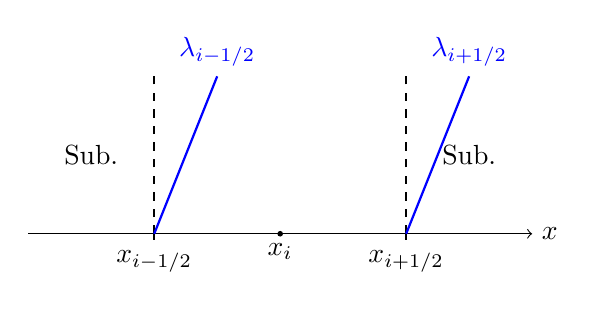
\begin{tikzpicture}[scale=0.4]
			  \draw[->]         (-8,0) -- (8,0)   node[right] {$x$};
			  \draw[thick,dashed]  (-4,0) -- (-4,5.);
			  \draw[thick,dashed] (4,0) -- (4,5.)  node[above] {};

			  \draw[thick] (-4,0.2)--(-4,-0.2) node[below] {$x_{i-1/2}$};
			  \draw[thick] (4,0.2)--(4,-0.2) node[below] {$x_{i+1/2}$};
			  \draw[fill=black] (0,0) circle (2pt) node[below]{$x_{i}$};

			  \draw (-6,2.5) node {Sub.};
			  \draw (6,2.5) node {Sub.};
			  \draw[color=blue, thick]  (-4,0) -- (-2,5)   node[above] {$\lambda_{i-1/2}$};
			  \draw[color=blue, thick]  (4,0) -- (6,5)     node[above] {$\lambda_{i+1/2}$};
			\end{tikzpicture}
	\label{fluvin_fluvout}
	}
	\hfill
	\subfloat[Supercritical input -- Supercritical output]{
		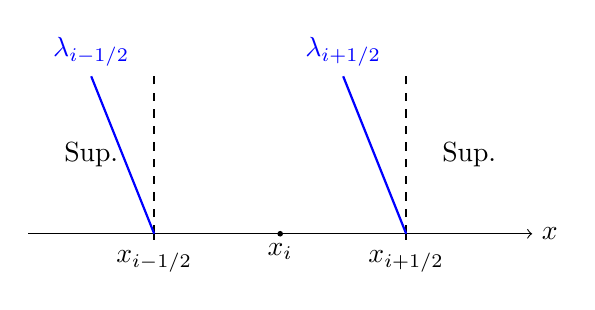
\begin{tikzpicture}[scale=0.4]
		  \draw[->]         (-8,0) -- (8,0)   node[right] {$x$};
		  \draw[thick,dashed]  (-4,0) -- (-4,5.);
		  \draw[thick,dashed] (4,0) -- (4,5.)  node[above] {};

		  \draw[thick] (-4,0.2)--(-4,-0.2) node[below] {$x_{i-1/2}$};
		  \draw[thick] (4,0.2)--(4,-0.2) node[below] {$x_{i+1/2}$};
		  \draw[fill=black] (0,0) circle (2pt) node[below]{$x_{i}$};

		  \draw (-6,2.5) node {Sup.};
		  \draw (6,2.5) node {Sup.};
		  \draw[color=blue, thick]  (-4,0) -- (-6,5)   node[above] {$\lambda_{i-1/2}$};
		  \draw[color=blue, thick]  (4,0) -- (2,5)     node[above] {$\lambda_{i+1/2}$};
		\end{tikzpicture}
		\label{torin_torout}
	}

	\subfloat[Subcritical input -- Supercritical output]{
		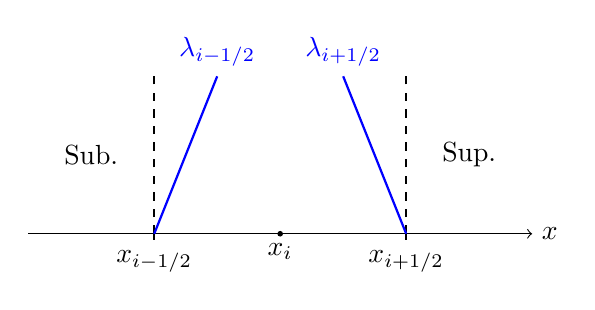
\begin{tikzpicture}[scale=0.4]
		  \draw[->]         (-8,0) -- (8,0)   node[right] {$x$};
		  \draw[thick,dashed]  (-4,0) -- (-4,5.);
		  \draw[thick,dashed] (4,0) -- (4,5.)  node[above] {};

		  \draw[thick] (-4,0.2)--(-4,-0.2) node[below] {$x_{i-1/2}$};
		  \draw[thick] (4,0.2)--(4,-0.2) node[below] {$x_{i+1/2}$};
		  \draw[fill=black] (0,0) circle (2pt) node[below]{$x_{i}$};

		  \draw (-6,2.5) node {Sub.};
		  \draw (6,2.5) node {Sup.};
		  \draw[color=blue, thick]  (-4,0) -- (-2,5)   node[above] {$\lambda_{i-1/2}$};
		  \draw[color=blue, thick]  (4,0) -- (2,5)     node[above] {$\lambda_{i+1/2}$};
		\end{tikzpicture}
		\label{fluvin_torout}
	}
	\hfill
	\subfloat[Supercritical input -- Subcritical output]{
		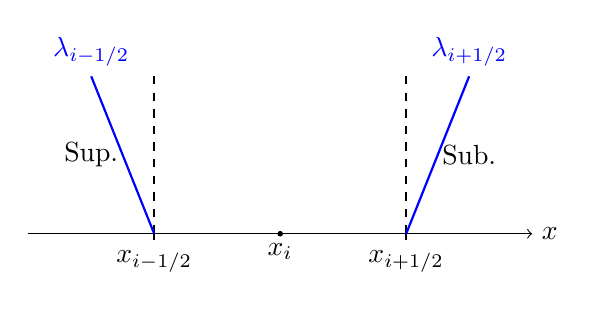
\begin{tikzpicture}[scale=0.4]
		  \draw[->]         (-8,0) -- (8,0)   node[right] {$x$};
		  \draw[thick,dashed]  (-4,0) -- (-4,5.);
		  \draw[thick,dashed] (4,0) -- (4,5.)  node[above] {};

		  \draw[thick] (-4,0.2)--(-4,-0.2) node[below] {$x_{i-1/2}$};
		  \draw[thick] (4,0.2)--(4,-0.2) node[below] {$x_{i+1/2}$};
		  \draw[fill=black] (0,0) circle (2pt) node[below]{$x_{i}$};

		  \draw (-6,2.5) node {Sup.};
		  \draw (6,2.5) node {Sub.};
		  \draw[color=blue, thick]  (-4,0) -- (-6,5)   node[above] {$\lambda_{i-1/2}$};
		  \draw[color=blue, thick]  (4,0) -- (6,5)     node[above] {$\lambda_{i+1/2}$};
		\end{tikzpicture}
		\label{torin_fluvout}
		}
	
	\caption{Different situations depending on the nature of the flow at the input and output of a cell from \cite{thesis_ung} - $\lambda$ is the wave velocity associated to the bed evolution.}
	\label{fig:allregcell}
\end{figure}

\nomenclature{$\lambda_i$}{Wave velocity associated to bed evolution in cell $i$ \nomunit{$m.s^{-1}$}}

Depending on the flow motion at the input and the output of the cell $i$, the variation of volume in the cell $i$ between two consecutive timsteps is computed from the following finite volume scheme :

\bequ
\begin{gathered}\label{eq:exner-scheme}
{(V)_i^{n+1} - (V)_i^n =}\\
\left\{
        \begin{array}{ll}
		  -\frac{\delta t}{\delta x} \left( (Q_s)_{i+1}^n - (Q_s)_{i}^n \right) & \textrm{if} \  (F_r)_{i-1/2} < 1 \  \textrm{and} \  (F_r)_{i+1/2} < 1 \  \textrm{(case \ref{fluvin_fluvout}),} \\
		  -\frac{\delta t}{\delta x} \left( (Q_s)_{i}^n - (Q_s)_{i-1}^n \right) & \textrm{if} \ (F_r)_{i-1/2} > 1 \  \textrm{and} \ (F_r)_{i+1/2} > 1 \  \textrm{(case \ref{torin_torout}),} \\
		  -\frac{\delta t}{2 \delta x} \left( (Q_s)_{i+1}^n - (Q_s)_{i-1}^n \right) & \textrm{if} \  (F_r)_{i-1/2} < 1 \  \textrm{and} \ (F_r)_{i+1/2} > 1 \  \textrm{(case \ref{fluvin_torout}),} \\
  0 & \textrm{if} \  (F_r)_{i-1/2} > 1 \  \textrm{and} \  (F_r)_{i+1/2} < 1 \  \textrm{(case \ref{torin_fluvout}).}
	\end{array}
	\right.
\end{gathered}
\eequ
where 
\begin{itemize}
	\item $(V)_i^n$ is the volume of sediment in the cell $i$ at the timestep $n$ ;
	\item $\delta t$ is the timestep ;
	\item $\delta x$ is the spacestep ;
	\item $(Q_s)_{i}^n$ is the solid discharge in the cell $i$ at the timestep $n$ given by the transport law ;
	\item $F_r$ is the Froude number defined such as \[ F_r = \dfrac{u}{\sqrt{gh_w}} \] with $h_w$ the water depth. 
\end{itemize}

\nomenclature{$h_w$}{Water depth \nomunit{$m$}}
\nomenclature{$F_r$}{Froude number \nomunit{$\emptyset$}}
\nomenclature{$V_i^n$ }{Volume of sediment in cell $i$ at the timestep $n$ \nomunit{$m^{3}$}}

The bottom elevation is then updated accordingly to the variation of volume computed above. The solid discharge $(Q_s)_{i}^n$ in cell $i$ at the timstep $n$ is computed with different transport formulae described below. 

\nomenclature{$Z_b$}{Bottom elevation \nomunit{$m$}}

Evolution of the river bottom is not applied in the same way for erosion and for deposition :
\begin{itemize}
 \item Evolution due to erosion is applied uniformely on all points of the river bottom located under the free surface ;
 \item Evolution due to deposition is applied horizontally (at constant elevation). For each horizontal deposition surface, the corresponding elevation is computed by linear interpolation of the curves generated by vertical discretization (cf Section \ref{planim}).
\end{itemize}

\begin{figure}[htb!]
    \centering
    \includegraphics[width=0.45\textwidth]{./graphics/erosion_deposition.png}
    \caption{Deposition and erosion mechanisms in \Cbedload}
    \label{fig:depo_ero}
\end{figure}

%%%%%%%%% FORMULES DE TRANSPORT %%%%%%%%%
\subsubsection{Transport formulae for the solid discharge}

Several transport formulae (cf Appendix \ref{app:formules_transport} for detailed expressions of these formulae) are available in \Cbedload :
\begin{itemize}
	\item Meyer-Peter and Müller (1948) \cite{MPM} : most commom transport formula, it is based on grain mouvement threshold concept and is valid for sediment sizes between 0.4 and \mbox{29 mm} and slopes between 0.4 and 2.4 \% \cite{lois_validite_recking}. This formula is not adapted to sand transport and is well known to underestimate solid transport at low flow rates. 
	\item Lefort (2015) : Lefort \cite{lefort} law was recently developed and validated over around 1 000 fields data and 3 400 laboratoy data. It is especially fitted for alpine rivers. This formula is valid for a wide range of slopes $I_f < 20\%$ and grain sizes $0.1\ mm < d_{50} < 55\ mm$. It was shown that this law remained relevant even with very high flow up to 28 000 m$^3/s$ \cite{lois_validite_recking}. This formula uses discharge which is easier to measure than bottom shear stress and therefore often offers a better estimation of transport rate. This formula is particularly suitable for gravel rivers but remains questionable for low flow.
	\item Recking (2013) \cite{recking2013} : This threshold formula was validated over 15 different reaches. This law is valid for grain sizes between 0.4 mm and 220 mm and a wide range of slopes $0.1\% < I_f < 7\%$\cite{lois_validite_recking}. It is especially suitable for gravel beds. 
	\item Recking (2015) \cite{recking2015}: In 2015, changes were proposed from the Recking formula to better take into account the effect of river morphologies on solid transport. The new formula was developped studying bedload measured in flumes (more than 12 data sets) and in the field (more than 133 data sets) \cite{recking2015}. 
\end{itemize}

%%%%%%%%%%%%%%%%%%%%%%% Slope stability %%%%%%%%%%%%%%%%%%%%%%%
\subsection{Slope stability}
\label{talus_th}

When emptying reservoirs, non-negligeable amount of sediment comes from sediment slide. Consequently, a simple sediment slide model was proposed in \courlis. It is available with both transport modules.

Slope stability is defined by two equilibrium slopes, one for underwater sediment $I_{stab, UN}$ and a second one for emerged sediment $I_{stab, EM}$.

\begin{CommentBlock}{Limit}
	Equilibrium slopes are given by the user but \courlis allows for only one value of ($I_{stab, UN}$, $I_{stab, EM}$) along the reach and for all sediment layers.
\end{CommentBlock}

Equilibrium slopes can be estimated thanks to soil measurements and empirical formulae proposed by Migniot \cite{Mig89} :
\bequ
	\tan I_{stab, UN} = k \tau_y
	\label{eq:stabUN}
\eequ

\bequ
	\tan I_{stab, EM} = k' \tau_y
	\label{eq:stabEM}
\eequ

where
\begin{itemize}
	\item $\tau_y$ is the intial stiffness of deposition;
	\item $k=0.01$ ;
	\item $k'=0.003$.
\end{itemize}

In all cross-section points, sediment slope is compared to the corresponding stability slope. If the sediment slope is larger than the stability slope, sediment crumbles to match the stability slope on this point.
Emerged sediment slide model is particularly relevant when emptying reservoirs as described above. On the other side, underwater sediment slide is essential to stabilize bed evolutions due to erosion. Indeed, \courlis can not reproduce channel enlargement, during flood for example, as free surface elevation and energy slope are supposed constant over the cross-section. Local shear stress is therefore maximal at the lower point where water depth is maximal and cause excessive erosion at the lower point and high lateral slopes as shown below on Figure \ref{fig:no_stab_model}. 

\begin{figure}[htb!]
	\centering
	\includegraphics[width=0.7\textwidth]{./graphics/chenal.png}
	\caption{Channel erosion with \courlis without slope stability model}
	\label{fig:no_stab_model}
\end{figure}

This model, based on a single threshold, remains simple and can still be improved. 

\begin{WarningBlock}{Warning}
	The user should also be aware that initial states can be unstable (initial geometry slopes higher than the stability slope) and therefore generate high, non-physical, sediment transport rates at the beginning of the simulation (mainly with \Csuspension). 
\end{WarningBlock}
%%%%%%%%%%%%%%%%%%%%%%% Coupling %%%%%%%%%%%%%%%%%%%%%%%
\subsection{Coupling between \courlis and \mascaret}
\label{coupling}
\begin{figure}[hbt!]
	\centering
	\includegraphics[width=\textwidth]{./graphics/coupling.png}
	\caption{Coupling between \courlis and \mascaret over a time $\Delta t = p \delta t_S = n \delta t_H$}
	\label{fig:coupling}
\end{figure}

The coupling between \courlis and \mascaret is weak. 
Shallow water equations are solved independently by the \mascaret kernel during $n$ timesteps. Hydraulics variables are used by \courlis for solid transport calculations and bed evolutions are given back to \mascaret after $p$ timesteps. Each code uses its own timestep $\delta t_H$ and $\delta t_S$. The hydraulics timestep $\delta t_H$ is chosen by the user while the solid transport timestep $\delta t_S$ is set such as :
$\Delta t = p \delta t_S = n \delta t_H$
The coupling parameters $p$ and $n$ are chosen by the user according to bed evolutions magnitude and speed. 

When the transcritical kernel of \mascaret (also called MASCARET) is used, the hydraulics timestep $\delta t_H$ can vary to match a Courant-Friedrich-Levy number set by the user (traditionally $CFL = 0.8$). 
This Courant-Friedrich-Levy number can reduce computational time as it adapts the hydraulics timestep to spacestep and hydraulics variables values at each iteration:
\bequ
	CFL = \left(  U+\sqrt{gH} \right)  \frac{\delta t_H}{\delta x}
	\label{eq:CFL}
\eequ
In this case, the sediment transport timestep $\delta t_S$ also varies during simulation accordingly. 

\nomenclature{$\delta t_H$}{Hydraulics timestep \nomunit{$s$}}
\nomenclature{$\delta t_S$}{Sediment transport timestep \nomunit{$s$}}




\newpage
%----------------------------------------------------------------------------------------
%	CHAPTER 1b: Evolution of the river cross-section
%----------------------------------------------------------------------------------------
\chapter{Evolution of cross-section}\label{chap1b}
\section{Introduction}

As we can see before, the sediment mass conservation equation, i.e. Exner equation \eqref{eq:exner}, only describes the time-evolution of $Z_b$ which is the bottom elevation (the lowest point of the river cross-section). More precisely, the numerical scheme \eqref{eq:exner-scheme} computes
\begin{equation}\label{eq:exner-sediment-volume}
\Delta V_i^{n+1} \equiv V_i^{n+1} - V_i^n
\end{equation}
the eroded/deposited volume of sediments at cell $i$ during the time $t^n$ to time $t^{n+1}$. As a consequent, an additional closure is needed in order to describe the evolution of river cross-section.

Several closures can be found in the literature. The simplest closure may be a {\em flat} deposition and an {\em uniform} erosion; the height of erosion at each point on the river cross-section can even be weighted in according with the efficient shear stress $\tau_{eff}$. An another one consists in applying an uniform evolution for both deposition and erosion cases.

Once the geometry of cross-sections are modified by erosion or deposition, the {\em planimetrage functions} -- vertical discretization of cross-sections -- need to be re-calculated at each time step
\begin{itemize}
\item $B(z)$: width of cross-section,
\item $S(z)$: area of cross-section,
\item $P(z)$: perimeter of cross-section,
\end{itemize}
corresponding to a given elevation $z$. As remarked before, this becomes costly for long-term simulations with a lot of bed evolutions (which can represent up to more than 90\% of the total calculation time of \courlis).

In the following, we are interested by the simple closures allowing direct analytic computation of planimetrage functions $B^{n+1}, S^{n+1}, P^{n+1}$ at time $t^{n+1}$ from time $t^n$ (available  functions $B^n, S^n, P^n$), or from the initial time $t^0$ (functions $B^0, S^0, P^0$ are given by \mascaret after initialization step).  The choice of these closures is given with the keyword \telkey{OPTION D'EVOLUTION DE PROFIL} or \telkey{OPTION FOR PROFILE EVOLUTION}.

\section{Option 1: uniform erosion -- flat deposition}

\subsection{Keywords}
\begin{itemize}
\item \telkey{OPTION FOR PROFILE EVOLUTION = 1} (default)
\end{itemize}

\subsection{Profile evolution}
Evolution of the river bottom is not applied in the same way for erosion and for deposition :
\begin{itemize}
 \item Evolution due to erosion is applied uniformely on all points of the river bottom located under the free surface ;
 \item Evolution due to deposition is applied horizontally (at constant elevation). For each horizontal deposition surface, the corresponding elevation is computed by linear interpolation of the curves generated by vertical discretization (cf Section \ref{planim}).
\end{itemize}

\begin{figure}[htb!]
    \centering
    \includegraphics[width=0.45\textwidth]{./graphics/erosion_deposition.png}
    \caption{Flat deposition and uniform erosion}
    \label{fig:depo_ero2}
\end{figure}

\subsection{Planimetrage functions}
wip

\section{Option 2: uniform erosion -- uniform deposition}

\subsection{Keywords}
\begin{itemize}
\item \telkey{OPTION FOR PROFILE EVOLUTION} = 2
\item \telkey{FILE FOR THE WIDTH OF EROSION} = largeur.xlim
\end{itemize}

\subsection{Profile evolution}
For a cross-section $i$, a value $B_i$ {\em width of erosion} or the positions $x_i^L, x_i^R$ on the left and the right river banks have to be prescribed in the \telkey{FILE FOR THE WIDTH OF EROSION}. The format of this later file is closely derived from that of geoCourlis as follows:

\begin{figure}[htb!]
\begin{verbatim}
Profil Bief_1 Profil_1 X1     Profil Bief_1 Profil_1 X1 [B1 or X1L X1R]
Profil Bief_1 Profil_2 X2     Profil Bief_1 Profil_2 X2 [B2 or X2L X2R]
...                           ...
\end{verbatim}
\caption{geoCourlis file (left) and (right) format of \telkey{FILE FOR THE WIDTH OF EROSION}.}
\end{figure}

The mechanism for erosion and deposition cases are illustrated on Fig. \ref{fig:option-uni-depo-ero}. The current geometry is derived from initial cross-section. In the case of erosion, the part of initial cross-section lying between $x^L$ and $x^R$ is uniformly displaced downward with a thickness $\delta z_i$. For the opposed case, this part of initial cross-section is uniformly moved upward by $\delta z_i$ and completed by horizontal jonctions at $x^L$ and $x^R$.

\begin{figure}[htb!]
    \centering
    \includegraphics[width=0.5\textwidth]{./graphics/option-uni-depot-ero.pdf}
    \caption{Uniform deposition and uniform erosion, with the brown curve corresponding to the initial profile}
    \label{fig:option-uni-depo-ero}
\end{figure}

\subsection{Planimetrage functions}
The planimetrage functions $B^{n+1}, S^{n+1}, P^{n+1}$ can be directly computed from those of initial time $B^0, S^0, P^0$.

First, we compute from $B^0$ the height $H_i$ associated to the given width of erosion $B_i$ by solving
\begin{equation}\label{eq:height-of-erosion}
  B_i=B_i^0(H_i).
\end{equation}

Given a volume of sediment $\Delta V_i^{n+1}$ (by \eqref{eq:exner-sediment-volume}), we next compute $\delta z_i$ the thickness of evolution and $B^{n+1}, S^{n+1}, P^{n+1}$ resulting from the conservation of sediment the cross-section:
\begin{itemize}
\item Erosion $(V_i^{n+1} \leq 0)$
  \begin{equation}\label{eq:thickness-of-erosion}
\Delta V_i^{n+1} = B_i\delta z_i\Delta x,
  \end{equation}
For a height $z$ from the bottom elevation $Z_b$,
  \begin{align*}
    	& S_i^{n+1}(z) = \left\{\begin{array}{lll}
	S_i^0(z) & \text{if} & z \leq H_i, \\
	S_i^0(H_i) + (z-H_i)B_i & \text{if} & H_i \leq z \leq H_i + \delta z, \\
	S_i^0(z-\delta z_i) + B_i\delta z_i & \text{else.}
	\end{array}\right. \\
	& B_i^{n+1}(z) = \left\{\begin{array}{lll}
	B_i^0(z) \hspace*{2cm} & \text{if} & z \leq H_i, \\
	B_i^0(H_i) & \text{if} & H_i \leq z \leq H_i + \delta z, \\
	B_i^0(z-\delta z_i) & \text{else.}
	\end{array}\right.\\
	& P_i^{n+1}(z) = \left\{\begin{array}{lll}
	P_i^0(z) & \text{if} & z \leq H_i, \\
	P_i^0(H_i) + 2(z-H_i) & \text{if} & H_i \leq z \leq H_i + \delta z_i, \\
	P_i^0(z-\delta z_i) + 2\delta z_i & \text{else.}
	\end{array}\right.
  \end{align*}

\item Deposition $(V_i^{n+1} > 0)$
   \begin{equation}\label{eq:thickness-of-deposition}
\Delta V_i^{n+1} = S_i^0(H_i + \delta z_i) - S_i^0(H).
   \end{equation}
For a height $z > 0$ from the bottom elevation $Z_b$,
   \begin{align*}
	& S_i^{n+1}(z) = \left\{\begin{array}{lll}
	S_i^0(z) & \text{if} & z \leq H_i, \\
	S_i^0(z+\delta z_i) - \Delta V_i^{n+1} & \text{else.}
	\end{array}\right. \\
	& B_i^{n+1}(z) = \left\{\begin{array}{lll}
	B_i^0(z) \hspace*{2cm} & \text{if} & z \leq H_i, \\
	B_i^0(z+\delta z_i) & \text{else.}
	\end{array}\right. \\
	& P_i^{n+1}(z) = \left\{\begin{array}{l}
	P_i^0(z) \hspace*{2cm} \text{if} \quad z \leq H_i, \\
	P_i^0(z+\delta z_i) + \Big[B_i^0(H_i+\delta z_i) - B_i\Big] - \Big[P_i^0(H_i+\delta z_i) - P_i^0(H_i)\Big].
	\end{array}\right.
	\end{align*}
\end{itemize}

\newpage
%----------------------------------------------------------------------------------------
%	CHAPTER 2: Pre-treatment
%----------------------------------------------------------------------------------------
\chapter{Pre-treatment}\label{chap2}
\section{PreCourlis}
wip

\section{Pretel}
wip

\newpage

%----------------------------------------------------------------------------------------
%	CHAPTER 3: The inputs
%----------------------------------------------------------------------------------------
\chapter{The inputs}\label{chap3}
To run a simulation, at least 4 files are needed :
\begin{itemize}
	\item The \cas for \courlis [Section \ref{cas_files}]
	\item The \xcas for \mascaret [Section \ref{cas_files}]
	\item The geometry file for \mascaret (\telfile{geometry.geo}) [Section \ref{geo_file}]
	\item The sediment layers file for \courlis (\telfile{geometry.geoC}) [Section \ref{geoC_file}]
\end{itemize}
Additional inputs can be used to specify liquid and solid boundary conditions or initial states. 

\section{The cas and xcas files}
\label{cas_files}
\subsection{Current set-up}
The \xcas containing \mascaret set up information can be adapted from \mascaret calculations or generated thanks to \fudaa (available at \url{www.opentelemac.org}). The reader can refer to the \mascaret guide for more information.

From a \mascaret file, the \courlis module is activated by modifying xml lines in the \xcas as described below :

\begin{figure}[htb!]
    \centering
    \includegraphics[width=0.9\textwidth]{./graphics/xcas_courlis.png}
    \caption{Changes in the \xcas to activate \courlis}
    \label{fig:xcas}
\end{figure}

First, the \courlis dictionary replaces the \mascaret one. Two lines are added to specify the activation of \courlis (\telkey{<optionCourlis>true</optionCourlis>}) and the name of the \courlis \cas (in this example called \telfile{courlis.cas}). 
These changes will call the \courlis routines with the parameters given in the corresponding \cas. \courlis can be shut off at any time by setting \telkey{<optionCourlis>false</optionCourlis>} resulting in a traditionnal \mascaret simulation. 

An example of an \xcas is given in Appendix \ref{app:xcas}. 

\begin{WarningBlock}{Warning}
	\fudaa provides an interface to generate \xcass but since \fudaa v7p2, the software is no longer supported. Consequently, 4 tags xml are missing from \xcass generated with \fudaa :
	\begin{itemize}
		\item	The \courlis dictionnary tag (Figure \ref{fig:xcas})
		\item 	The \courlis option tag (Figure \ref{fig:xcas})
		\item	The \courlis key file tag (Figure \ref{fig:xcas})
		\item 	The uncentered scheme option tag for the permanent kernel of \mascaret (Figure \ref{fig:xcas_decentrement})
	\end{itemize}
	If a \fortran error (\verb"At line 531 of file .../pretrait.f90") appears while running \mascaret with SARAP it may be that the recently developed option of uncentered scheme for this kernel has not been added to the \xcas.
\end{WarningBlock}

\begin{figure}[htb!]
    \centering
    \includegraphics[width=0.8\textwidth]{./graphics/decentrement_xcas.png}
    \caption{Changes in the \xcas to add the uncentered option (set to \telkey{TRUE} to activate it)}
    \label{fig:xcas_decentrement}
\end{figure}

The \cas put in the \xcas controls \courlis parameters.
\courlis keywords, gathered in this file, are presented in the next sections.
An example is given in Appendix \ref{app:cas}. 

\subsection{Coming set-up}
Soon the code will only parse \xcass, one for \mascaret and one for \courlis, and no longer one \xcas for \mascaret and one \cas for \courlis. Nevertheless, thanks to \python script, the user will have the choice to launch the calculation with two \cass or two \xcass.

This improvement will make \mascaret parameters more readable and intuitive to facilitate its use.
\xcass can be converted to \cas via the command \\
\verb|manip_cas.py xcas2cas_1d <my_xcas_file.xcas> <output_cas_file.cas>|.

\begin{CommentBlock}{Warning}
	The keywords are not yet all translated in the dictionnary. So, in v8p3, this conversion will make a mixed english/french \cas !
\end{CommentBlock}

%%%%%%%%%%%%%%%%%%% GEOMETRY %%%%%%%%%%%%%%%%%%%%%
\section{Geometry and sediment layers}
\label{sedi_layers}

\subsection{The .geo file}
\label{geo_file}

The geometry file contains the initial bottom elevations of the reach, i.e. the initial elevation of the interface between the bottom and the water. 
Simple geometries can be generated thanks to \fudaa. Extraction of profiles from bathymetric measurements can be done thanks to \precourlis\footnote{In QGIS : \url{https://plugins.qgis.org/plugins/PreCourlis/} or GitHub : \url{https://github.com/msecher/PreCourlis}}.
While using \courlis, no mesh can be generated during simulation. That is why, unlike \mascaret, the cross-sections must be interpolated in pre-treatment.
If the space step of the geometry is not sufficient, interpolation can also be done with \precourlis.

\begin{CommentBlock}{Warning}
	It is recommended to avoid as much as possible vertical walls in geometry when using \courlis. Indeed, some approximations are done by \mascaret when lateral walls are vertical and hydraulics errors will be amplified by \courlis calculations. 
\end{CommentBlock}

\subsection{The .geoC file}
\label{geoC_file}

The \courlis geometry file contains the initial elevations of the different sediment interfaces. 

For each cross-section, the first column corresponds to the bottom layer as specified in the \telfile{geo file}. The next columns correspond to the different interfaces between sediment layers (as shown below). The last column corresponds to a non-erodable substratum (hard bottom). 
With the suspension module, two virtual layers are commonly set to represent sand and silt transport i.e. the initial width of these two layers is null. A third layer can be added to represent sediment already present in the initial step. This configuration corresponds to 4 interfaces in the \telfile{geoC file} as represented below
When modeling bedload, only one layer is useful and therefore 2 interfaces are given in the \telfile{geoC file} as represented below. 

\begin{figure}[htb!]
    \centering
    \includegraphics[width=\textwidth]{./graphics/geo_files.png}
    \caption{Examples of one cross-section in the \telfile{geo and geoC files} for (a) bedload and (b) suspension simulations}
    \label{fig:geo_files}
\end{figure}

\section{Optional inputs}
\label{optional_inputs}

Hydraulics boundary conditions are often written in an external file, for example \telfile{hydrograph.loi} at the upstream boundary and \telfile{elevation.loi} at the downstream boundary. Initial free surface elevations can also be given in an external file for example called \telfile{init.lig}. All external files names are specified in the \xcas. The reader can refer to the \mascaret guide for more information.\\

Similarly, sediment concentrations at boundaries can be given to \courlis from external files, for example \telfile{qs.loi}. The corresponding \telkey{LOI CONC X MODE D''ENTREE} keyword, with \telkey{X} the law number, should be set to \telkey{1} in the \cas (and conversely to \telkey{2} if the information is given directly in the \cas). The name of the files are then given by \telkey{LOI CONC X FICHIER}.\\

Initial concentrations for \Csuspension can be set into an external file : 
\begin{itemize}
	\item \telkey{MODE D'ENTREE DES CONCENTRATIONS INITIALES POUR COURLIS = 1} (by default)
	\item \telkey{FICHIER DES CONCENTRATIONS INITIALES POUR COURLIS} : the external file name
\end{itemize}

In addition, sediment characteristics can also be given in an external file :
\begin{itemize}
	\item \telkey{MODE D''ENTREE DES CARACTERISTIQUES SEDIMENTAIRES = 1} (by default)
	\item \telkey{FICHIER DES CARACTERISTIQUES SEDIMENTAIRES} : the external file name
\end{itemize}

\begin{WarningBlock}{French-English keywords}
	Keywords were first developed in French. Translation of keywords in English has been started (\telfile{sources/mascaret/mascaret.dico}) but is not yet available in the code. Consequently, the following sections will present the French keywords and the corresponding English keywords when they are available in \courlis v8p3 (listed in the \verb|dico_Courlis.txt| generated when launching a \courlis simulation).
\end{WarningBlock}


\newpage

%----------------------------------------------------------------------------------------
%	CHAPTER 4: General Setup
%----------------------------------------------------------------------------------------
\chapter{General setup}\label{chap4}
\section{Sediment transport}
\subsection{Transport mechanism}
The modelling of either bedload or suspended load is done thanks to :
\begin{itemize}
	\item \telkey{OPTION CHARRIAGE} or \telkey{BEDLOAD OPTION} : Set to \telkey{TRUE} or \telkey{VRAI} for \Cbedload (default=\telkey{FALSE})
	\item \telkey{OPTION SUSPENSION} or \telkey{SUSPENSION OPTION} : Set to \telkey{TRUE} or \telkey{VRAI} for \Csuspension (default=\telkey{FALSE})
\end{itemize}

If \Cbedload is chosen, the transport law is defined by \telkey{LOI DE TRANSPORT} :
\begin{itemize}
	\item \telkey{1} : Meyer-Peter and Müller (1948), value by default (\S \ref{app:MPM})
	\item \telkey{2} : Lefort (2015) (\S \ref{app:lefort})
	\item \telkey{3} : Recking (2013) (\S \ref{app:recking2013})
	\item \telkey{4} : Recking (2015) (\S \ref{app:recking2015})
\end{itemize}

If \Csuspension is chosen, sand calculations can be disabled by setting \telkey{CALCUL AVEC SABLE} to \telkey{FALSE} (by default sand calculations are allowed).

\subsection{Sediment properties}
Sediment properties can be given in an external file (by default, \telkey{MODE D''ENTREE DES CARACTERISTIQUES SEDIMENTAIRES = 1}) or directly in the \cas : \telkey{MODE D''ENTREE DES CARACTERISTIQUES SEDIMENTAIRES = 2} (cf \S \ref{optional_inputs}). \\

Using a \cas is recommanded.

\section{Geometry set up}
\label{geo_set_up}

The \telfile{geoC file} name is given by \telkey{FICHIER DE GEOMETRIE COURLIS}.
The corresponding number of sediment layers should be specified in \telkey{NOMBRE DE COUCHES}.\\

The \telfile{geo file} name is given in the \xcas file to \mascaret. It is also indicated at the beginning of the \cas file :
\begin{itemize}
	\item \telkey{FICHIER DES MOT-CLES} = your \xcas between single quotation mark
	\item \telkey{PROGRAMME PRINCIPAL} = \verb|'princi.f'|
	\item \telkey{FICHIER DE GEOMETRIE} = your \telfile{geo file.geo} between single quotation mark
\end{itemize}

\section{Initial conditions}

Initial bottom elevations are given in the \telfile{geoC and geo files} (see section above).
Initial free surface elevation can be given in an external file or computed by \mascaret.

Initial concentrations in \Csuspension can be given in an external file (cf \S \ref{optional_inputs}) or directly in the \cas (\telkey{MODE D'ENTREE DES CONCENTRATIONS INITIALES POUR COURLIS = 2}):
\begin{itemize}
	\item \telkey{NOMBRE DE POINTS DECRIVANT LES CONC INITIALES POUR COURLIS} : Number of points
	\item \telkey{ABSCISSES DES CONC INI} : List of points' abscissae (along $x$), for example \verb|0.0;1.0;2.0|
	\item \telkey{CONCENTRATION EN VASE INI} : List of points' silt concentrations in g/L, for example \verb|0.0;0.0;0.0|
	\item \telkey{CONCENTRATION EN SABLE INI} : List of points' sand concentrations in g/L, for example \verb|0.0;0.0;0.0|
\end{itemize}

\section{Boundary conditions}

Liquid boundary conditions are specified in the \xcas.

Solid boundary conditions are specified in the \cas. Variations of sediment concentrations with time define boundary conditions laws which are given either in an external file (especially for large number of points, cf \S \ref{optional_inputs}) or directly in the \cas :
\begin{itemize}
	\item \telkey{NOMBRE DE LOIS DE CONCENTRATION } : Number of different laws
	\item \telkey{LOI CONC NUMERO X} : Law ID, \telkey{X} is an integer from 1 to 15
	\item \telkey{LOI CONC X NOM} : Law name of law \telkey{X} between single quotation mark, for example 'Constant concentration'
	\item \telkey{LOI CONC X MODE D'ENTREE} : Input type for law \telkey{X}, external file \telkey{1} or directly in \cas \telkey{2} (cf \S \ref{optional_inputs})
\end{itemize}

If an external file is used, the corresponding file name should be written in :
\begin{itemize}
	\item \telkey{LOI CONC X FICHIER} : External file name for law \telkey{X} between single quotation mark (cf \S \ref{optional_inputs})
\end{itemize}

Otherwise, the law \telkey{X} should be define thanks to the following keywords :
\begin{itemize}
	\item \telkey{LOI CONC X NOMBRE DE POINTS} : Number of points
	\item \telkey{LOI CONC X TEMPS} : List of points' time in seconds, for example \verb|0.0;3600.0|
	\item \telkey{LOI CONC X CONCENTRATION} : List of points' concentrations in g/L. for example \verb|3.14;3.14|
\end{itemize}

Finally, laws affected to the upstream boundary are defined by :
\begin{itemize}
	\item \telkey{NUMERO LOI CONC AMONT VASE} : Law ID for silt upstream inflow
	\item \telkey{NUMERO LOI CONC AMONT SABLE} : Law ID for sand upstream inflow
\end{itemize}

Similarly, it is possible to affect laws to lateral inflows (i.e. set a sediment inflow from affluents where a liquid inflow has already been added in \mascaret) in the same order as they have been given in the \xcas:
\begin{itemize}
	\item \telkey{NUMERO LOI CONC APPORT VASE} : Law IDs for silt lateral inflow, for example \verb|3;4| to refer to the third law for the first affluent and the fourth law for the second affluent.
	\item \telkey{NUMERO LOI CONC APPORT SABLE}: Law IDs for sand lateral inflow, for example \verb|5;6|
\end{itemize}

With \Cbedload, it is possible to set the upstream solid discharge through an equilibrium slope. A law must still be given to the upstream boundary but it will not be taken into account. \\

This option relies on the following keywords : \telkey{CONCENTRATION AMONT CALCULEE AVEC PENTE EQUILIBRE} set to \telkey{TRUE} to use an equilibrium slope instead of the values given by the law and \telkey{PENTE EQUILIBRE AMONT} to specify this equilibrium slope, by default this keyword is equal to 0.01 for a 1\% slope. \\

By default, concentration are given without voids but by setting \telkey{CONCENTRATION AMONT SANS LES VIDES} to \telkey{FALSE}, voids will be taken into account for the upstream law.

\newpage

%----------------------------------------------------------------------------------------
%	CHAPTER 5: Physical parameters
%----------------------------------------------------------------------------------------
\chapter{Physical parameters}\label{chap5}
\section{Sediment layers}

According to the geometrical set up given in \S \ref{geo_set_up}, the sediment layers are described by the following keywords :
\begin{itemize}
	\item \telkey{NOM DES COUCHES} : List of layers names, for example \verb|'Silt deposition';| \verb|'Sand deposition';'Mixed sediment layer'| or \verb|'Gravel bed'|
	\item \telkey{CONCENTRATION DES COUCHES} : List of layers concentration, for example \verb|1000.0;|\verb|1000.0;1000.0| or \verb|2650|
\end{itemize}

\subsection{\Cbedload}
Several grain diameters can be defined accordingly to the beload formula used :
\begin{itemize}
	\item \telkey{D84} : Diameter for which 84\% of grains are smaller (coarse fraction) in meters
	\item \telkey{DIAMETRE MOYEN} : Mean diameter in meters
	\item \telkey{D16} : Diameter for which 16\% of grains are smaller (fine fraction) in meters
	\item \telkey{D50 DES SABLES} : Median diameter in meters
	\item \telkey{POROSITE} : Porosity, by default 0.25.
\end{itemize}

\begin{CommentBlock}{Uknown grain sizes}
  If \telkey{D84}, \telkey{DIAMETRE MOYEN} or \telkey{D16} are set to 0.0, the following formulae are used to dertermine there values automatically:
  \begin{itemize}
    \item $d_{84}=2.1 d_{50}$,
    \item $d_{m}=1.1 d_{50}$,
    \item $d_{16}=0.5 d_{50}$.
  \end{itemize}
\end{CommentBlock}

\subsection{\Csuspension}
\begin{itemize}
	\item \telkey{POURCENTAGE DE SABLE} : List of layers sand proportion from 0 to 100, for example
\verb| 0.0;100.0;50.0|
	\item \telkey{D50 DES SABLES} : List of median diameters for sands in meters in each layers, for example \verb|1.0;700.E-6;700.E-6|
	\item \telkey{VITESSE DE CHUTE DES SABLES} : List of settling velocity for sands in each layers
	\item \telkey{VITESSE DE CHUTE DES VASES} : Settling velocity for silts
	\item \telkey{CONTRAINTE CRITIQUE D'EROSION DES VASES} : List of critical shear stresses for silt erosion $\tau_{c, erosion}$ for each layer, for example \verb|5.0;5.0;5.0|
	\item \telkey{CONTRAINTE CRITIQUE DE DEPOT DES VASES} : Critical shear stress for silt deposition $\tau_{c, deposition}$
	\item \telkey{COEFFICIENT DE PARTHENIADES} : List of Partheniades coefficient for each layers
\end{itemize}

\section{Friction parameters}

The friction coefficients (cf \S \ref{sediment_transport_th}) are given by the following keywords :
\begin{itemize}
	\item \telkey{STRICKLER DE PEAU} : List of skin friction coefficient per layer
	\item \telkey{STRICKLER TOTAL} : List of bottom friction coefficient per layer
\end{itemize}

\section{Slope stability model}

The slope stablility model is described in \S \ref{talus_th}. The corresponding keywords are :
\begin{itemize}
  \item \telkey{SEDIMENT SLIDE OPTION} : option to activate the option when it set to \telkey{TRUE} (by default, it is set to \telkey{FALSE})
  \item \telkey{MODELE DE RUPTURE DES TALUS} : 1 (this keyword should always define to this value)
	\item \telkey{PENTE DE STABILITE DES TALUS IMMERGES} : Equilibrium slope for underwater sediment $I_{stab, UN}$ in \%, for example 0.8
	\item \telkey{PENTE DE STABILITE DES TALUS EMERGES} : Equilibrium slope for emerged sediment $I_{stab, EM}$ in \%, for example 0.5
\end{itemize}


\newpage
%----------------------------------------------------------------------------------------
%	CHAPTER 6: Numerical parameters
%----------------------------------------------------------------------------------------
\chapter{Numerical parameters}\label{chap6}
% Numerical parameters found in suspension examples :
% COEFFICIENT DE DIFFUSION DES VASES = 0
% CONVECTION DES TRACEURS POUR COURLIS = vrai
% OPTION DE CONVECTION POUR LES TRACEURS POUR COURLIS = 4
% ORDRE DU SCHEMA DE CONVECTION VOLUMES FINIS POUR COURLIS = 3
% PARAMETRE W DU SCHEMA DE CONVECTION VOLUMES FINIS POUR COURLIS = 0
% LIMITEUR DE PENTE DU SCHEMA VOLUMES FINIS POUR COURLIS = vrai

\section{Vertical discretization and clipping parameters} \label{planim}
The vertical discretization step is set in the \xcas.

To limit the calls to the vertical discretization process, two options are proposed in \courlis :
\begin{itemize}
	\item \telkey{CLIP ABSOLU SUR L'EVOLUTION} or \telkey{ABSOLUTE CLIP EVOLUTION} : The vertical discretization process is done every time bottom variations are higher than the clipping value in meters. For example, \telkey{ABSOLUTE CLIP EVOLUTION = 0.05} means the vertical discretization process will take place every time bottom variations are higher than 5 centimenters. It is by default equal to \telkey{1e-5} m.
	\item The second option suggests a clipping depending on the water depth. If the \telkey{CLIPPING OPTION} is set to \telkey{TRUE} (by default, \telkey{CLIPPING OPTION = FALSE}), the vertical discretization process is called every time bottom variation is more than a given percentage (between 0 and 1) specified in \telkey{CLIP EVOLUTION}. For example, \telkey{CLIP EVOLUTION = 0.05} means the vertical discretization process will happen every time bottom variation represents more than 5\% of the water depth.
\end{itemize}
For now, no option has been shown to be more efficient than the other.
The clipping value can be adapted for each simulation and a compromise between errors generated by this clipping and computational time should be found.

To start, a clipping value of 1\% is recommended.

\section{Local slope option} \label{local_slope_opt}

The energy slope value used in bedload transport laws can be computed from the head values along the reach (computed by \mascaret) or from the Strickler formula (Equation \ref{eq:strickler}) using the mean water depth, the section geometry, the liquid discharge and the Strickler coefficient.

Historically, the first method was used in \courlis. Yet, in some cases, this option led to high bed instabilities caused by the hydraulics computed by \mascaret, sometimes locally perturbed.

That is why the option \telkey{PENTE LOCALE} was developped.

\begin{WarningBlock}{Recommendation}
	It is highly recommended to set \telkey{PENTE LOCALE = TRUE}.
\end{WarningBlock}

\section{Coupling parameters}\label{coupling_param}

The coupling parameters described in \S \ref{coupling} $n$ and $p$ correspond to the keywords \telkey{NOMBRE D'ITERATIONS HYDRAULIQUE} for the hydraulics number of iterations $n$ and \telkey{NOMBRE D'ITERATIONS SEDIMENTO} for the sediment transport number of iterations $p$.

\section{Uncentered scheme for SARAP kernel}\label{uncentered}
When using the permanent kernel of \mascaret, SARAP, an option is available in the \xcas to use an uncentered scheme on the energy slope (see Figure \ref{fig:xcas_decentrement}).

Traditionnally, the energy slope term $J$ in the shallow water equations (Equation \ref{eq:shallow}) was approximated by upstream and downstream values.
This option replaces this scheme to consider only the upstream value as described below :
\bequ
	    J = \frac{2}{\frac{1}{J_{downstream}}+\frac{1}{J_{upstream}}} \rightarrow J = J_{upstream}
\eequ

The use of this uncentered scheme with \Cbedload has shown good results and seems to be less mesh-sensitive.

\section{Printouts}\label{printouts}

The outputs files names (see \S \ref{outputs} for description of these files) are given with the following keywords :

\begin{itemize}
	\item \telkey{FICHIER LISTING COURLIS} : The listing file name, for example \telfile{results.listingcourlis} ;
	\item \telkey{FICHIER RESULTATS PROFIL EN LONG} : The longitudinal profile results file name, for example \telfile{results.plong} ;
	\item \telkey{FICHIER RESULTATS PROFIL EN TRAVERS} : The cross-sections results file name, for example \telfile{results.ptravers} ;
\end{itemize}

For the values printed in the listing, different printouts are available :

\begin{itemize}
	\item \telkey{IMPRESSION DES PARAMETRES SEDIMENTAIRES} : Printouts of sediment characteristics
	\item \telkey{IMPRESSION DES INTERFACES SEDIMENTAIRES} : Printouts of sediment layers interfaces
	\item \telkey{IMPRESSION DES PARAMETRES DE COUPLAGE} : Printouts of coupling parameters
	\item \telkey{IMPRESSION DES CONC INITIALES POUR COURLIS} : Printouts of initial concentrations
	\item \telkey{IMPRESSION DES LOIS DE CONCENTRATION} : Printouts of boundary conditions laws
	\item \telkey{IMPRESSION DES APPORTS SEDIMENTAIRES} : Printouts of sediment inflows
\end{itemize}

An important parameter to limit computational time and the size of the results files is the printout step. For \mascaret, printouts periods are given in the \xcas. For \courlis, several keywords are given to limit printouts during calculation :

\begin{itemize}
	\item \telkey{PAS D'IMPRESSION COURLIS} : Period in number of sediment timesteps for \courlis printouts in the \telfile{listing file}
	\item \telkey{PAS DE STOCKAGE POUR LE PROFIL EN LONG} : Period in number of sediment timesteps for \courlis printouts in the \telfile{plong file}
	\item \telkey{PAS DE STOCKAGE POUR LE PROFIL EN TRAVERS} : Period in number of sediment timesteps for \courlis printouts in the \telfile{ptravers file}
\end{itemize}

The boolean \telkey{DEBUG CHARRIAGE} permits to print bedload values in the listing for each section at each iteration to detect inconsistencies.

\newpage
%----------------------------------------------------------------------------------------
%	CHAPTER 7: Calculation run
%----------------------------------------------------------------------------------------
\chapter{Calculation run}\label{chap7}
\section{First run}

From your working folder, in the same way as for hydraulics simulations with \mascaret, the user should call the \mascaret script:
\lstset{language=bash,
        basicstyle=\scriptsize\ttfamily}

\begin{lstlisting}[escapechar=|]
[bash:] mascaret.py <your_xcas_file.xcas>
\end{lstlisting}

An example of a \Cbedload simulation on a Debian 10 machine is given below :
\lstset{language=TelemacCas}
\begin{lstlisting}
Loading Options and Configurations
~~~~~~~~~~~~~~~~~~~~~~~~~~~~~~~~~~~~~~~~~~~~~~~~~~~~~~~~~~~~~~~~~~~~~~~~

(*@\color{codegreen} < COURLIS VERSION >@*)

Running your CAS file(s) for:
~~~~~~~~~~~~~~~~~~~~~~~~~~~~~~~~~~~~~~~~~~~~~~~~~~~~~~~~~~~~~~~~~~~~~~~~



~~~~~~~~~~~~~~~~~~~~~~~~~~~~~~~~~~~~~~~~~~~~~~~~~~~~~~~~~~~~~~~~~~~~~~~~

S10.gfortran.dyn: 
    

    +> Gfortran compiler 8.3.0 with open_mpi for a Debian 10

    +> root:    (*@\color{codegreen} <your root folder>@*)
    +> module: ad / api / artemis / bief
               damocles  / gaia  / gretel  / hermes
               identify_liq_bnd  / khione  / mascaret  / nestor
               parallel  / partel  / postel3d  / sisyphe
               special  / stbtel  / telemac2d  / telemac3d
               tomawac / waqtel


~~~~~~~~~~~~~~~~~~~~~~~~~~~~~~~~~~~~~~~~~~~~~~~~~~~~~~~~~~~~~~~~~~~~~~~~


... processing the steering file

... checking parallelisation

... handling temporary directories
~+> Creating FichierCas.txt
                                                                               
... checking the executable


Running your simulation(s) :
~~~~~~~~~~~~~~~~~~~~~~~~~~~~~~~~~~~~~~~~~~~~~~~~~~~~~~~~~~~~~~~~~~~~~~~~



In (*@\color{codegreen} <your simulation folder>@*):
mpirun -np 1 (*@\color{codegreen} <your root folder>@*)/builds/S10.gfortran.dyn/bin/mascaret


 Fichiercas : FichierCas.txt

 TELEMAC-MASCARET V8P2R0beta == Copyright (C) 2000-2020 EDF-CEREMA ==

 Data File : (*@\color{codegreen} <your xcas file.xcas>@*)

 Clip Evolution = (*@\color{codegreen} <non absolute clipping value>@*)

 Pente locale : T

 Parametres utilises seulement pour les formules de transport de Recking et de Lefort
 D84 = (*@\color{codegreen} < >@*)
 Diametre moyen = (*@\color{codegreen} < >@*)

 Parametre utilise seulement pour la formule de transport de Lefort
 D16 = (*@\color{codegreen} < >@*)

 Bedload option : T  (*@\color{codegreen} Bedload simulation@*)

 Suspension option : F

 sediment slide option : F

 planim clipping option : F

 absolute clipping = (*@\color{codegreen} <absolute clipping value>@*)

 bedload transport law is (*@\color{codegreen} <transport law>@*)
 Study name : (*@\color{codegreen} <your study name>@*)

 Hydraulic statistics (prior solve phase)
    ------ Geometric parameters ------
    Number of reach(es)       =            1
    Number of cross-sections  =           (*@\color{codegreen} <nb sections>@*)
    Number of open boundaries =            2
    Number of junction(s)     =            0
    Number of inflow(s)       =            0
    Number of lateral weir(s) =            0
    Number of storage area(s) =            0
    Number of link(s)         =            0
    Number of dam(s)/weir(s)  =            0
    ------ Numerical parameters ------
    Number of 1D nodes (mesh) =           (*@\color{codegreen} <nb sections>@*)
    Computation Kernel        =            1
    Initial time step         =      	(*@\color{codegreen} <dt>@*)
    Variable time step?       =            0
    Simulation time           =      	(*@\color{codegreen} <t max>@*)

 (*@\color{PantoneRed}OptionCourlis T@*)
 Start the Simulation...
\end{lstlisting}

\section{Calculation continuation}

wip


\begin{WarningBlock}{Warning}
	When updating your version of \courlis, make sure to delete the precedent \telfile{dictionnary file} before running your simulation again.
\end{WarningBlock}


\newpage
%----------------------------------------------------------------------------------------
%	CHAPTER 8: The outputs
%----------------------------------------------------------------------------------------
\chapter{The outputs}\label{outputs}
\section{Mascaret outputs}
The hydraulics variables values are given in the \telfile{opt file} like in \mascaret simulations. 
Hydraulics variables are also printed in the \telfile{lis file}.  

\section{Dictionnary}
All keywords available for \courlis for a given version are listed in the \telfile{dictionnary file}.

\section{The listingcourlis file}\label{listing_courlis}

The \telfile{listingcourlis file} 
wip

\section{The plong file}\label{plong}
wip

\section{The ptravers file}\label{ptravers}
wip

\section{The damoc files}
wip
% Errors in Fortran in damocles files

\newpage
%----------------------------------------------------------------------------------------
%	CHAPTER 9: Post-treatment
%----------------------------------------------------------------------------------------
\chapter{Post-treatment}\label{chap9}
\section{Fudaa-mascaret}
wip

\section{Pretel}
wip


\newpage

%----------------------------------------------------------------------------------------
%	---------- APPENDICES ----------
%----------------------------------------------------------------------------------------
\appendix
%----------------------------------------------------------------------------------------
%	APPENDIX A: Transport formulae
%----------------------------------------------------------------------------------------
\chapter{Transport formulae for \courlis-bedload}
\label{app:formules_transport}
%%%%%%%%%%%%%%%%%%%%%%%%%%%% MPM %%%%%%%%%%%%%%%%%%%%%%%%%%%%
\section{Meyer-Peter \& Müller (1948)}
\label{app:MPM}

The most common formula, and still currently used nowadays, is the Meyer-Peter \& Müller \cite{MPM} formula also noted MPM. 
It was elaborated from bedload experiments in flumes for median grain sizes between 0.4 à 29 mm. 
Sediment transport is computed above a critical stress $\tau_c = 0.047$ and the solid transport rate is computed from :
\bequ
    Q_s = \frac{C_{MPM}}{1-n} B\sqrt{R g d_{50}^3} \left(\theta^*-\theta_c \right)^{\frac{3}{2}}
\eequ
where the adimensional efficient shear stress $\theta^*$ is defined as
\bequ
	\theta^* = \left(\frac{K}{K_p}\right)^{\frac{3}{2}} \theta
\eequ
\begin{itemize}
	\item $C_{MPM}$ is a coefficient for the MPM formula. In \courlis, $C_{MPM} = 8$ ;
	\item $n$ represents the sediment porosity, by default $n=0.25$. Its value can be changed by the user via the option \telkey{POROSITE};
	\item $d_{50}$ is the median grain diameter ;
	\item $R$ the relative reduced density $R=\frac{\rho_s}{\rho_w}-1$.
\end{itemize}

The Shields parameter $\theta$ is computed from 
\bequ
    \label{eq:shields}
    \theta = \frac{U^2}{RK^2R_h^{\frac{1}{3}}d_{50}} 
\eequ

\nomenclature{$C_{MPM} $}{Meyer-Peter \& Müller coefficient \nomunit{$\emptyset$}}
\nomenclature{$U$}{Average velocity across section \nomunit{$m.s^{-1}$}}
\nomenclature{$d_m$}{Mean diameter \nomunit{$m$}}
\nomenclature{$R$}{Relative reduced density \nomunit{$\emptyset$}}
\nomenclature{$\rho_s$}{Sediment density \nomunit{$kg.m^{-3}$}}
\nomenclature{$\rho_w$}{Water density \nomunit{$kg.m^{-3}$}}
\nomenclature{$Q_s$}{Solid discharge \nomunit{$m^3.s^{-1}$}}
\nomenclature{$B$}{Bed width \nomunit{$m$}}
\nomenclature{$d_{50}$}{Median diameter \nomunit{$m$}}
\nomenclature{$K_p$}{Skin friction coefficient \nomunit{$m^{\frac{1}{3}}.s^{-1}$}}
\nomenclature{$\theta$}{Shields number \nomunit{$\emptyset$}}
\nomenclature{$\tau$}{Shear stress \nomunit{$Pa$}}
\nomenclature{$u^*$}{Vitesse de frottement sur le fond \nomunit{$m.s^{-1}$}}
\nomenclature{$\tau_c$}{Critical shear stress \nomunit{$Pa$}}
\nomenclature{$\theta_c$}{Critical Shields number \nomunit{$\emptyset$}}
\nomenclature{$\theta^*$}{Adimensional efficient shear stress \nomunit{$\emptyset$}}
\nomenclature{$\tau^*$}{Efficient shear stress  \nomunit{$Pa$}}
\nomenclature{$\Phi^*$}{Einstein number \nomunit{$\emptyset$}}
\nomenclature{$n$}{Porosity \nomunit{$\emptyset$}}
\nomenclature{$\nu$}{Kinematic viscosity of water \nomunit{$Pa.s$}}
\nomenclature{$d_{16}$}{Diameter for which 16\% of grains are smaller (fine fraction) \nomunit{$m$}}
\nomenclature{$d_{84}$}{Diameter for which 84\% of grains are smaller (coarse fraction) \nomunit{$m$}}
\nomenclature{$d_{90}$}{Diameter for which 90\% of grains are smaller \nomunit{$m$}}

The MPM formula is not fit for sand transport nor high slopes problems. Moreover, it often underestimates gravel transport during periods of low flow \cite{lefort}.

%%%%%%%%%%%%%%%%%%%%%%%%%%%% LEFORT %%%%%%%%%%%%%%%%%%%%%%%%%%%%
\section{Lefort (2015)}
\label{app:lefort}

In Lefort \cite{lefort} equation, an adimensional diameter $d_m^*$ is defined such as:
\bequ
	d_m^* = d_m {\left[\frac{gR}{\nu^2}\right]}^{\frac{1}{3}}
\eequ
where $\nu$ is the water kinematic viscosity.

The transition discharge $Q_0$ which separates partiel bedload from general bedload is chosen such as :
\bequ
 	\frac{Q_0}{B\sqrt{g(Rd_{m})^3}} = C(d_m^*) \left(\frac{d_m}{B}\right)^{\frac{1}{3}} \left(\frac{K}{K_p}\right)^{-0.5} J^{-m_0}
\eequ
with $C(d_m^*)$ a function to describe the Shields stress variation with the mean grain diameter:
\bequ
	C(d_m^*) = 0.0444 \left[1+\frac{15}{1+d_m^*}-1.5\exp{\left(-\frac{d_m^*}{75}\right)}\right] 
\eequ
The shear stress increase with slope is done thanks to the exponent $m_0$ such as 
\bequ
	 m_0 = 1.6 +0.06 \log_{10}(J)
\eequ

The solid discharge is then estimated as :
\bequ
	Q_s = \frac{1.7}{1-n}\: Q \: J^m \frac{R+1}{R^{1.65}} \left[0.5\left(\frac{d_{84}}{d_{50}}\frac{d_{50}}{d_{16}}\right)\right]^{0.2} C_{dune} \frac{F(Q)}{(R+1)(1-n)}
\eequ
with $m = 1.8 +0.08\log_{10}(J)$

The term $0.5 \left(\frac{d_{84}}{d_{50}}\frac{d_{50}}{d_{16}}\right)$ relates to the particle size range.

The dune correction coefficient $C_{dune}$ serves to model the increase in friction due to the development and the transport of dunes. It is set for grain diameters above 0.6 mm. According to Lefort \cite{lefort}, it has little influence on the results. 
\bequ
	 C_{dune} = \left\{
        \begin{array}{ll}
            1-1.4\exp\left(-0.9 \left(\frac{K}{K_p}\right)^2\left(\frac{Q}{Q_0}\right)^{0.5}\right) \qquad \textrm{if}\quad d_m^*<14 \quad \textrm{and} \quad \frac{K}{K_p}<0.63, \\
            1 \qquad \textrm{otherwise}\\
        \end{array}
    \right.
\eequ

The discharge function $F$ describes the partial bedload of fine particles and general tranport, first bedload and then bedload and suspended load, via the following expression :
\bequ
	F(Q) = \left\{
        \begin{array}{ll}
            0.06 \: C_M \: \frac{Q}{Q_0} \qquad \textrm{if}\quad Q<Q_0, \\
            {\left[0.6{\left(1-0.938{\left(\frac{Q_0}{Q}\right)}^{0.284}\right)}^{1.66}\right]}^{m_z} \qquad \textrm{otherwise}\\
        \end{array}
    \right.
\eequ
with $m_z$ the add-on exponent for solid discharge during the transition between bedload and suspension:
\bequ
	m_z = \left\{
        \begin{array}{ll}
            1+\frac{0.38}{{d_m^*}^{0.45}} {\left(\frac{Q}{B\sqrt{gd_m^3}}\right)}^{0.192} \qquad \textrm{if}\quad Q>3.4Q_0, \\
            1 \qquad \textrm{otherwise}\\
        \end{array}
    \right.
\eequ
and $C_M$ a reduction factor of transport for partial bedload :

\bequ
	C_M = \left\{
        \begin{array}{ll}
            \frac{1}{200}\left(\frac{Q}{B\sqrt{gJd_{m}^3}}+2.5\right) \qquad \textrm{if}\quad \frac{Q}{B\sqrt{gJd_{m}^3}}<200, \\
            1 \qquad \textrm{otherwise}\\
        \end{array}
    \right.
\eequ

When the ratio $\frac{K}{K_p}$ is unknown, an alternative is suggested and can be activated in \courlis with the boolean \telkey{ROUGHNESS RATIO WITH QSTAR FOR LEFORT}.

When set to \telkey{TRUE}, the friction coefficient ratio is given by :
\bequ
	\frac{K}{K_p} = \left\{
        \begin{array}{ll}
            0.75 {\left(\frac{Q}{200B\sqrt{gJd_{84}^3}} \right)}^{0.23}  \qquad \textrm{if}\quad \frac{Q}{B\sqrt{gJd_{84}^3}}<200, \\
            0.75 \qquad \textrm{otherwise}\\
        \end{array}
    \right.
\eequ

%%%%%%%%%%%%%%%%%%%%%%%%%%%% RECKING 2013 %%%%%%%%%%%%%%%%%%%%%%%%%%%%
\section{Recking (2013)}
\label{app:recking2013}

The Recking \cite{recking2013} transport law is based on the surface diameter $d_{84}$ to characterize the bed friction and its ratio with the median diameter to characterize the particle size range. 

A mobility stress $\theta^*_m$ is defined, to separate partial bedload from general bedload. This parameter is also called the Recking number \cite{lefort}. 
This mobility stress is supposed constant for sands ($d_m < 2mm : \theta^*_m=0.045$) and is evaluated for other particles by :
\bequ
	\theta^*_m = \left(5J + 0.06\right){\left(\frac{d_{84}}{d_{50}}\right)}^{4.4\sqrt{J}-1.5}
\eequ
The associate Shields stress is computed by :
\bequ
	\theta_{84}^* = \frac{J}{Rd_{84} \left(\frac{2}{B}+74 p^{2.6}(gJ)^p \left(\frac{Q}{B}\right)^{-2p} d_{84}^{3p-1}\right)}
\eequ
with \[p = \left\{
        \begin{array}{ll}
            0.2275 \qquad \textrm{if}\quad \frac{Q}{B\sqrt{gJd_{84}^3}}<100, \\
            0.3025 \qquad \textrm{otherwise}\\
        \end{array}
    \right.\]
An Einstein number is then defined from this two stresses by :
\bequ
	 \Phi = \frac{14{\theta_{84}^{*}}^{2.5}}{1+{\left(\frac{\theta^*_m}{\theta_{84}^*}\right)}^4}
\eequ
Finally, the solid discharge can be written as :
\bequ
	Q_s = \frac{B}{1-n} \Phi \sqrt{gRd_{84}^3}
\eequ

%%%%%%%%%%%%%%%%%%%%%%%%%%%% RECKING 2015 %%%%%%%%%%%%%%%%%%%%%%%%%%%%
\section{Recking (2015)}
\label{app:recking2015}

In 2015, new estimations for the mobility stress were added to the Recking formula to discriminate riffle-pools and alternate bars (where it depends on $\frac{d_{84}}{d_{50}}$) from other morphologies (especially rivers with flat beds and narrow channels)\cite{recking2015}. Examples of those different morphologies are shown in Figure \ref{fig:morpho_recking2015}. 

For these latter, $\theta^*_m$ expression becomes :
\bequ
	\theta^*_m = 1.5 J^{0.75}
	\label{eq:recking2015_others}
\eequ
For sand bed rivers, this choice does not matter because the Shield number is generally high enough so errors generated by taking the average stress over the section remains negligeable. 

In \courlis, the expression of $\theta^*_m$ is set by the option \telkey{MORPHOLOGY OPTION RECKING 2015}. By default, it is equal to 1 for riffle-pools and alternate bars but it can be set to 2 to use the expression above (Equation \ref{eq:recking2015_others}).

The Shields number is computed by default from the discharge (\telkey{SHIELDS SHEAR STRESS WITH DISCHARGE FOR RECKING 2015 = TRUE}) :

\bequ
\theta_{84}^* = 0.015\frac{J}{R} {\left(\frac{Q}{B\sqrt{gJd_{84}^3}}\right)}^{2p} \frac{1}{p^{2.5}}
\eequ
with \[p = \left\{
        \begin{array}{ll}
            0.23 \qquad \textrm{if}\quad \frac{Q}{B\sqrt{gJd_{84}^3}}<100, \\
            0.31 \qquad \textrm{otherwise}\\
        \end{array}
    \right.\]
Otherwise, the Shields number is computed from the hydraulic radius :
\bequ
	\theta_{84}^* = \frac{JR_h}{Rd_{84}}
\eequ

\begin{figure}[htb!]
    \centering
    \includegraphics[width=0.45\textwidth]{./graphics/recking2015.jpg}
    \caption{(a) A step-pool stream (Tinée), (b) a plane-bed stream (Byasse), (c) a riffle-pool stream (Drac), (d) a braided stream (Bléone), (e) a sand-bed river (Loire). © S. Rodrigez. from Recking et al. \cite{recking2015}}
    \label{fig:morpho_recking2015}
\end{figure}

\newpage
%----------------------------------------------------------------------------------------
%	APPENDIX B: Examples of cas and xcas files
%----------------------------------------------------------------------------------------
\chapter{Examples of cas and xcas files}
\section{The \xcas}
\label{app:xcas}
\lstinputlisting[language=xml]{../../../examples/courlis/lefort/depot_lefort_sarap.xcas}

\section{The \cas}
\label{app:cas}
\subsection{\Cbedload example}
\lstinputlisting[language=TelemacCasRed]{../../../examples/courlis/lefort/depot_lefort_courlis_sarap.cas}
\subsection{\Csuspension example}
\lstinputlisting[language=TelemacCasRed]{../../../examples/courlis/Garonne/hydro_courlis.cas}
\newpage
%---------------------------------------------------------------------------
% Bibliography
%---------------------------------------------------------------------------

\bibliographystyle{plainnat}
%\bibliography{../../data/biblio}
\bibliography{./latex/courlis_user_guide.bib}
\end{document}
